\documentclass[10pt]{article}
\usepackage[utf8]{inputenc}
\usepackage[T1]{fontenc}
\usepackage{amsmath}
\usepackage{amsfonts}
\usepackage{amssymb}
\usepackage[version=4]{mhchem}
\usepackage{stmaryrd}
\usepackage{bbold}
\usepackage{graphicx}
\usepackage[export]{adjustbox}
\graphicspath{ {./images/} }

d\begin{document}
% \section*{Computable Functions}
% In this part of the course, we study several formal definitions of algorithm. These definitions are equivalent, providing different ways of describing the notion of computable function.

% \section*{Algorithms, informally}
% People tried to find an algorithm to solve Hilbert's\\
% Entscheidungsproblem, without success.\\
% A natural question was then to ask whether it was possible to prove that such an algorithm did not exist. To ask this question properly, it

% \section*{Slide 1}
%  was necessary to provide a formal definition of algorithm.Common features of the (historical) examples of algorithms:

% \begin{itemize}
%   \item finite description of the procedure in terms of elementary operations;
%   \item deterministic, next step is uniquely determined if there is one;
%   \item procedure may not terminate on some input data, but we can recognise when it does terminate and what the result will be.
% \end{itemize}

% We will initially explore definitions of algorithm which are closer to how machines compute. We first give a formal definition of register machine, which provides a simple description of a computing machine. We then give a definition of Turing machine, which is more complicated description of a computing machine. Although more complicated, every computer scientist should know about Turing machines! Finally, we give a definition of Church's lambdacalculus. This provides a completely different way of describing computation which is much nearer to the notion of function rather than the notion of computing machine. What is amazing is that these different definitions are actually equivalent.

% \section*{Algorithms as Special Functions}
% Turing and Church's equivalent definitions of algorithm capture the notion of computable function: an algorithm expects some input, does some calculation and, if it terminates, returns a unique result.\\
% Slide 2\\
% We first study register machines, which provide a simple definition of algorithm. We describe the universal register machine and introduce the halting problem, which is probably the most famous example of a problem that is not computable.

% We then move to Turing machines and Church's $\lambda$-calculus.

% \section*{Register Machines}
% The register machine gets its name from its one or more uniquely addressed registers, each of which holds a natural number. There are several versions of register machines. We are using the Minski register machines. The work on register machines occurred in the 1950s and 1960s. One motivation was that people were trying to show that Hilbert's 10th problem on Diophantine equations was undecidable. This was finally cracked in 1970s using Turing machines, and a simpler proof was given in the 1980s using register machines. Register machines are (apparently) particularly suited to constructing Diophantine equations [Matiyasevich].

% \section*{Register Machines}
% \section*{Definition}
% A register machine (sometimes abbreviated to RM) is specified by:

% \begin{itemize}
%   \item finitely many registers $R_{0}, R_{1}, \ldots, R_{n}$, each capable of storing a natural number;\\
% Slide 4
%   \item a program consisting of a finite list of instructions of the form label : body where, for $i=0,1,2, \ldots$, the $(i+1)^{\text {th }}$ instruction has label $L_{i}$. The instruction body takes the form:
% \end{itemize}

% \begin{center}
% \begin{tabular}{|ll|}
% \hline
% $R^{+} \rightarrow L^{\prime}$ & add 1 to contents of register $R$ and jump to instruction labelled $L^{\prime}$ \\
% \hline
% $R^{-} \rightarrow L^{\prime}, L^{\prime \prime}$ & if contents of $R$ is $>0$, then subbract 1 and jump to $L^{\prime}$, else jump to $L^{\prime \prime}$ \\
% \hline
% $H A L T$ & stop executing instructions \\
% \hline
% \end{tabular}
% \end{center}

% \section*{Example}
% \section*{Slide 5}
% \begin{center}
% \begin{tabular}{|l|l|}
% \hline
% Registers & Example Computation \\
% \hline
% $R_{0} R_{1} R_{2}$ & $L_{i} \quad R_{0} \quad R_{1} \quad R_{2}$ \\
% \hline
% Program & $\begin{array}{llll}0 & 0 & 1 & 2\end{array}$ \\
% \hline
%  & $1 \begin{array}{llll}1 & 0 & 0 & 2\end{array}$ \\
% \hline
% $L_{0}: R_{1}^{-} \rightarrow L_{1}, L_{2}$ & $0 \begin{array}{llll}0 & 1 & 0 & 2\end{array}$ \\
% \hline
% $L_{1}: R_{0}^{+} \rightarrow L_{0}$ & $2 \begin{array}{llll}2 & 1 & 0 & 2\end{array}$ \\
% \hline
% $L_{2}: R_{2}^{-} \rightarrow L_{3}, L_{4}$ & $3 \begin{array}{llll}3 & 1 & 0 & 1\end{array}$ \\
% \hline
% $L_{3}: R_{0}^{+} \rightarrow L_{2}$ & $\begin{array}{llll}2 & 2 & 0 & 1\end{array}$ \\
% \hline
% $L_{4}: H A L T$ & $2-3-0$ \\
% \hline
%  & $4 \quad 300$ \\
% \hline
% \end{tabular}
% \end{center}

% Exercise Consider the following program, acting on registers $R_{0}, R_{1}, R_{2}, R_{3}$ :

% $$
% \begin{array}{|l|}
% \hline \text { Program } \\
% L_{0}: R_{1}^{-} \rightarrow L_{1}, L_{6} \\
% L_{1}: R_{2}^{-} \rightarrow L_{2}, L_{4} \\
% L_{2}: R_{0}^{+} \rightarrow L_{3} \\
% L_{3}: R_{3}^{+} \rightarrow L_{1} \\
% L_{4}: R_{3}^{-} \rightarrow L_{5}, L_{0} \\
% L_{5}: R_{2}^{+} \rightarrow L_{4} \\
% L_{6}: H A L T \\
% \hline
% \end{array}
% $$

% Give the example computation starting from initial configuration $(0,2,3,0)$.

% \section*{Graphical representation}
% \begin{itemize}
%   \item One node in the graph for each instruction label : body, with the node labelled by the register of the instruction body; notation $[L]$ denotes the register of the body of label $L$
%   \item Arcs represent jumps between instructions
% \end{itemize}

% Slide 10

% \begin{itemize}
%   \item Initial instruction START.
% \end{itemize}

% \begin{center}
% \begin{tabular}{|ll|}
% \hline
% Instruction & Representation \\
% \hline
% $R^{+} \rightarrow L$ & $R^{+} \longrightarrow[L]$ \\
% \hline
% $R^{-} \rightarrow L, L^{\prime}$ &  \\
%  & $\left.R^{-} \longrightarrow L\right]$ \\
%  &  \\
% \hline
% $H A L T$ & $H A L T$ \\
% \hline
% $\left.L_{0}\right]$ &  \\
% \hline
% \end{tabular}
% \end{center}

% Slide 11

% \section*{Example}
% \begin{center}
% \begin{tabular}{|l|}
% \hline
% Registers \\
% $R_{0} R_{1} R_{2}$ \\
% Program \\
% $L_{0}: R_{1}^{-} \rightarrow L_{1}, L_{2}$ \\
% $L_{1}: R_{0}^{+} \rightarrow L_{0}$ \\
% $L_{2}: R_{2}^{-} \rightarrow L_{3}, L_{4}$ \\
% $L_{3}: R_{0}^{+} \rightarrow L_{2}$ \\
% $L_{4}: H A L T$ \\
% \hline
% \end{tabular}
% \end{center}

% \begin{center}
% 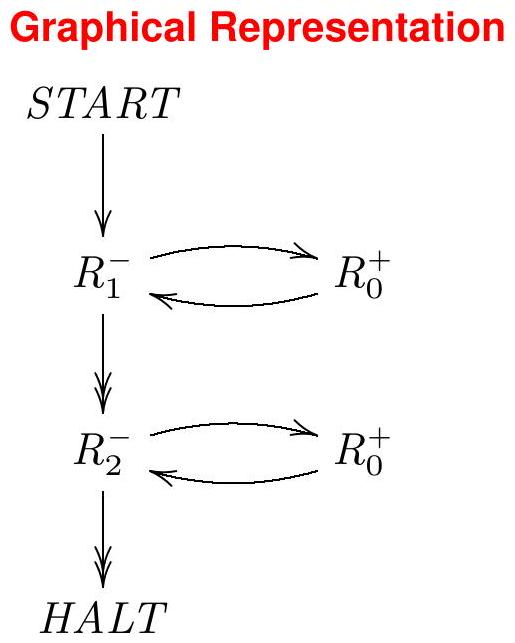
\includegraphics[max width=\textwidth]{2025_05_09_e840a83aab7eebacdc7fg-08}
% \end{center}

% Claim: starting from initial configuration $(0,0, x, y)$, this machine's computation halts with configuration $(4, x+y, 0,0)$.

% The graphical representation is a bit confusing. There is one node in the graph for each instruction label : body. However, the nodes are only labelled with the registers of the instruction bodies. For example, in slide 10, we have two nodes labelled $R_{0}^{+}$. The top node corresponds to the instruction $L_{1}: R_{0}^{+} \rightarrow L_{0}$, and the bottom node to $L_{3}: R_{0}^{+} \rightarrow L_{2}$. The initial instruction $S T A R T$ is essential, as the graphical representation looses the sequential ordering of instructions.\\
% Exercise Recall the following program acting on registers $R_{0}, R_{1}, R_{2}, R_{3}$ :

% $$
% \begin{array}{|l|}
% \hline \text { Program } \\
% L_{0}: R_{1}^{-} \rightarrow L_{1}, L_{6} \\
% L_{1}: R_{2}^{-} \rightarrow L_{2}, L_{4} \\
% L_{2}: R_{0}^{+} \rightarrow L_{3} \\
% L_{3}: R_{3}^{+} \rightarrow L_{1} \\
% L_{4}: R_{3}^{-} \rightarrow L_{5}, L_{0} \\
% L_{5}: R_{2}^{+} \rightarrow L_{4} \\
% L_{6}: H A L T \\
% \hline
% \end{array}
% $$

% What is the graphical representation of this program?

% \section*{Partial functions}
% Register machine computation is deterministic: in any non-halting configuration, the next configuration is uniquely determined by the program.

% Slide 12\\
% So the relation between initial and final register contents defined by a register machine program is a partial function...

% Definition A partial function from a set $X$ to a set $Y$ is specified by any subset $f \subseteq X \times Y$ satisfying

% $$
% (x, y) \in f \text { and }\left(x, y^{\prime}\right) \in f \text { implies } y=y^{\prime} .
% $$

% \section*{Partial Functions}
% \section*{Notation}
% \begin{itemize}
%   \item " $f(x)=y$ " means $(x, y) \in f$
%   \item " $f(x) \downarrow$ " means $\exists y \in Y(f(x)=y)$
% \end{itemize}

% Slide 13

% \begin{itemize}
%   \item " $f(x) \uparrow$ " means $\neg \exists y \in Y(f(x)=y)$
%   \item $X \rightharpoonup Y=$ set of all partial functions from $X$ to $Y$\\
% $X \rightarrow Y=$ set of all (total) functions from $X$ to $Y$\\
% Definition. A partial function from a set $X$ to a set $Y$ is total if it satisfies
% \end{itemize}

% $$
% f(x) \downarrow
% $$

% for all $x \in X$.

% \section*{Computable functions}
% Definition. The partial function $f \in \mathbb{N}^{n} \rightarrow \mathbb{N}$ is (register machine) computable if there is a register machine $M$ with at least $n+1$

% Slide 14 registers $R_{0}, R_{1}, \ldots, R_{n}$ (and maybe more) such that for all $\left(x_{1}, \ldots, x_{n}\right) \in \mathbb{N}^{n}$ and all $y \in \mathbb{N}$,\\
% the computation of $M$ starting with $R_{0}=0, R_{1}=x_{1}, \ldots$, $R_{n}=x_{n}$ and all other registers set to 0 , halts with $R_{0}=y$\\
% if and only if $f\left(x_{1}, \ldots, x_{n}\right)=y$.

% The I/O convention is somewhat arbitrary: in the initial configuration, registers $R_{1}, \ldots, R_{n}$ store the function's arguments (with all others zeroed); in the halting configuration, register $R_{0}$ stores it's value (if any). Notice that there may be many different register machines that compute the same partial function $f$.

% \section*{Example}
% Slide 15\\
% 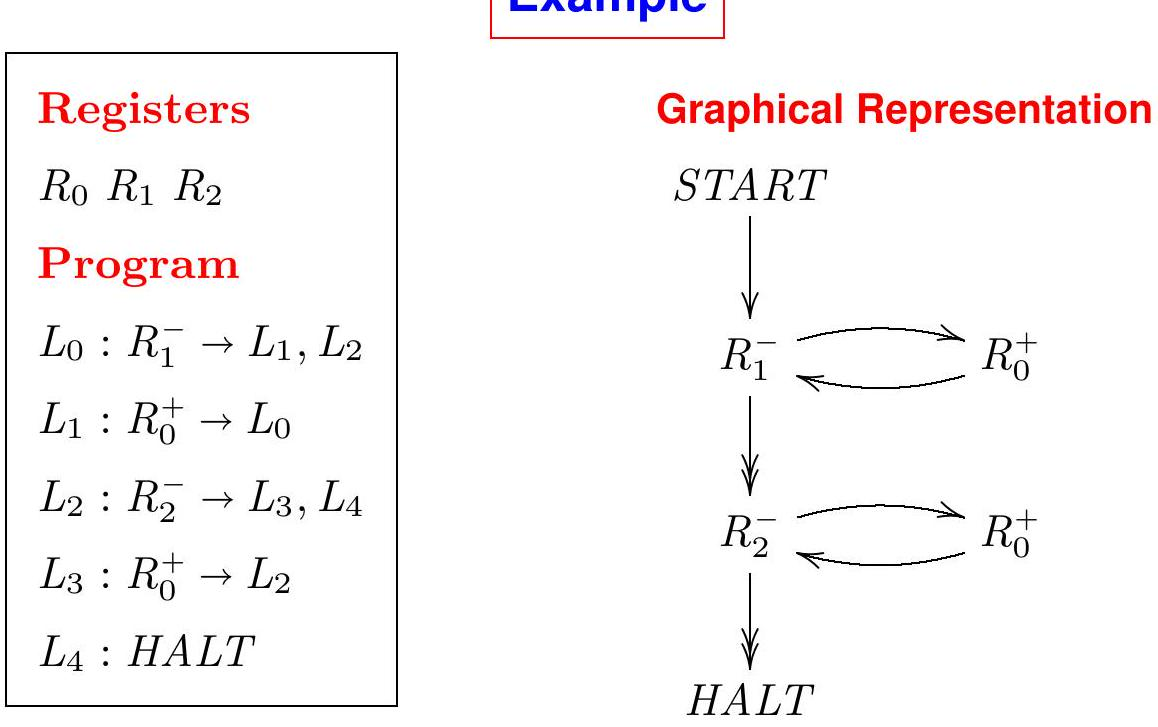
\includegraphics[max width=\textwidth, center]{2025_05_09_e840a83aab7eebacdc7fg-11}

% If the machine starts with registers $\left(R_{0}, R_{1}, R_{2}\right)=(0, x, y)$, then it halts with registers $\left(R_{0}, R_{1}, R_{2}\right)=(x+y, 0,0)$.

% The notation is a little confusing. The slide states that, if the machine starts with registers $\left(R_{0}, R_{1}, R_{2}\right)=(0, x, y)$, then it halts with registers $\left(R_{0}, R_{1}, R_{2}\right)=(x+y, 0,0)$. This description focusses on registers, and demonstrates that $f(x, y) \triangleq x+y$ is computable. (The notation $f(x, y) \triangleq x+y$ means that $f(x, y)$ 'is defined to be equal to' $x+y$.) Compare this description with the description using configurations in slide 11: starting from initial configuration ( $0,0, x, y$ ), this machine's computation halts with configuration $(4, x+y, 0,0)$. This description also gives information about the initial and final labels. The configuration $(0,0, x, y)$ means that the first component is the initial label 0 , the second component is initially set to zero and will eventually give the final answer when the computation halts, and the third and fourth components provide the two input values of the function. From configuration $(0,0, x, y)$, this machine's computation halts with configuration $(4, x+y, 0,0)$.

% Multiplication $f(x, y) \triangleq x y$ is computable

% Slide 16\\
% 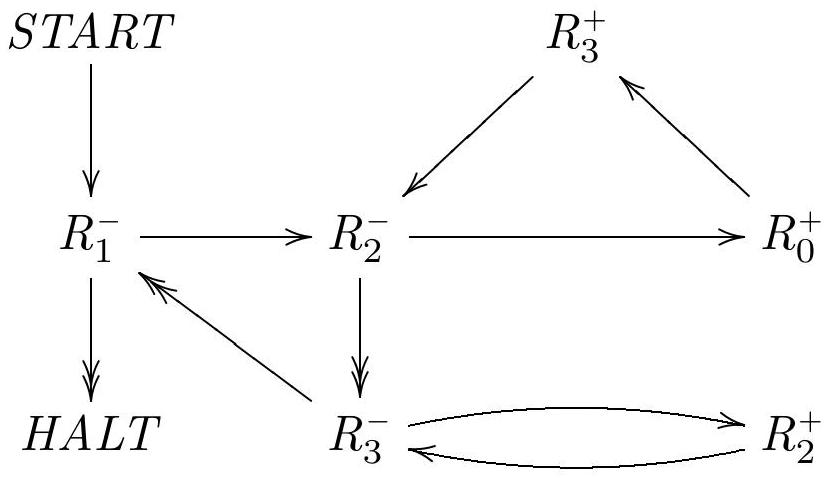
\includegraphics[max width=\textwidth, center]{2025_05_09_e840a83aab7eebacdc7fg-12}

% If the machine starts with registers $\left(R_{0}, R_{1}, R_{2}, R_{3}\right)=(0, x, y, 0)$, then it halts with registers $\left(R_{0}, R_{1}, R_{2}, R_{3}\right)=(x y, 0, y, 0)$.

% Exercise Construct a register machine that computes the function $f(x, y) \triangleq x+y$.\\
% The following arithmetic functions are all computable. The proofs are left as exercises.

% \begin{enumerate}
%   \item Projection: $p(x, y) \triangleq x$
%   \item Constant: $c(x) \triangleq n$
%   \item Truncated subtraction: $x-y \triangleq \begin{cases}x-y & \text { if } y \leq x \\ 0 & \text { if } y>x\end{cases}$
%   \item Integer division: $x$ div $y \triangleq \begin{cases}\text { integer part of } x / y & \text { if } y>0 \\ 0 & \text { if } y=0\end{cases}$
%   \item Integer remainder: $x \bmod y \triangleq x \perp y(x$ div $y)$
%   \item Exponentiation base 2: $e(x) \triangleq 2^{x}$
%   \item Logarithm base 2: $\log _{2}(x) \triangleq \begin{cases}\text { greatest } y \text { such that } 2^{y} \leq x & \text { if } x>0 \\ 0 & \text { if } x=0\end{cases}$
% \end{enumerate}

% \section*{Coding Programs as Numbers}
% So far, we have only seen how to write simple arithmetical operations as register-machine programs. The Turing/Church solution of the Entscheidungsproblem and the Halting problem uses the fundamentally important idea that (formal descriptions of) algorithms can be the data on which algorithms act. Recall the following slide from lecture 1.

% \section*{The Halting Problem}
% The Halting Problem is the decision problem with

% \begin{itemize}
%   \item the set $S$ of all pairs $(A, D)$, where $A$ is an algorithm and $D$ is some input datum on which the algorithm is designed to operate;
%   \item the property $A(D) \downarrow$ holds for $(A, D) \in S$ if algorithm $A$ when applied to $D$ eventually produces a result: that is, eventually halts.
% \end{itemize}

% Turing and Church's work shows that the Halting Problem is unsolvable (undecidable): that is, there is no algorithm $H$ such that, for all $(A, D) \in S$,

% $$
% \begin{aligned}
% H(A, D) & =1 \quad A(D) \downarrow \\
% & =0 \quad \text { otherwise }
% \end{aligned}
% $$

% To realise this idea of algorithms being used as input data in the context of Register Machines, we have to be able to code register-machine programs as numbers. (In general, such codings are often called Gödel numberings.) To do this, first we have to code pairs of numbers and lists of numbers as numbers. There are many ways to do this. We fix upon one way.

% \section*{Numerical Coding of Pairs}
% \section*{Definition}
% For $x, y \in \mathbb{N}$, define $\left\{\begin{array}{l}\langle x, y\rangle \triangleq 2^{x}(2 y+1) \\ \langle x, y\rangle \triangleq 2^{x}(2 y+1)-1\end{array}\right.$

% \section*{Slide 18}
% Example $27=0 \mathrm{~b} 11011=\langle\langle 0,13\rangle=\langle 2,3\rangle$

% \section*{Result}
% $《-,-\rangle$ gives a bijection between $\mathbb{N} \times \mathbb{N}$ and\\
% $\mathbb{N}^{+}=\{n \in \mathbb{N} \mid n \neq 0\}$.\\
% $\langle-,-\rangle$ gives a bijection between $\mathbb{N} \times \mathbb{N}$ and $\mathbb{N}$.\\
% Recall the definition of bijection from discrete maths.

% The notation 0b11011 is sometimes used to emphasise that the number, in this case 11011, is in binary. We will also use the notation $0 \mathrm{~b} x$ for $x \in \mathbb{N}$ to denote the binary number of $x$. We investigate a few examples of $\langle\langle x, y\rangle$ for small examples of $x$ and $y$ :

% $$
% \begin{aligned}
% & \langle 0,0\rangle=1 \quad\langle 1,0\rangle=2 \quad\langle 2,0\rangle=4 \quad\langle 3,0\rangle=8 \\
% & \langle 0,1\rangle=3 \quad\langle 1,1\rangle=6 \quad\langle 2,1\rangle=12 \quad \ldots \\
% & \langle 0,2\rangle=5 \quad\langle 1,2\rangle=10 \quad 《 2,2\rangle=20 \quad \ldots \\
% & \langle 0,3\rangle=7 \quad \ldots
% \end{aligned}
% $$

% \section*{Numerical Coding of Pairs}
% \section*{Definition}
% For $x, y \in \mathbb{N}$, define $\left\{\begin{array}{l}\langle x, y\rangle \triangleq 2^{x}(2 y+1) \\ \langle x, y\rangle \triangleq 2^{x}(2 y+1)-1\end{array}\right.$

% \section*{Slide 19}
% \section*{Sketch Proof of Result}
% It is enough to observe that

% $$
% \begin{array}{|l|l|}
% \hline 0 \mathrm{~b}\langle\langle x, y\rangle\rangle & =\begin{array}{|l|l|l|}
% \hline 0 \mathrm{~b} y & 1 & 0 \cdots 0 \\
% \hline 0 \mathrm{~b}\langle x, y\rangle & \quad x \text { number of } 0 \mathrm{~s} \\
% \hline
% \end{array} \begin{array}{|l|l|l|}
% \hline 0 \mathrm{~b} y & 0 & 1 \cdots 1 \\
% \hline
% \end{array} x \text { number of } 1 \mathrm{~s}
% \end{array}
% $$

% where $0 \mathrm{~b} x \triangleq x$ in binary. $\triangleq$ means 'is defined to be'.

% To show that

% $$
% \begin{array}{|l|l|l|}
% \hline 0 \mathrm{~b}\langle x, y\rangle & 0 \mathrm{~b} y & 1 \\
% \underbrace{0 \cdots 0}_{x 0 s} \\
% \hline
% \end{array}
% $$

% observe that $\langle x, y\rangle \triangleq 2^{x}(2 y+1)=2^{x+1} y+2^{x}$.\\
% To show $\left\langle\langle-,-\rangle: \mathbb{N} \times \mathbb{N} \rightarrow \mathbb{N}^{+}\right.$is one-to-one, assume that $\left\langle\left\langle x_{1}, y_{1}\right\rangle=\right.$ $\left\langle\left\langle x_{2}, y_{2}\right\rangle\right.$, and either $x_{1} \neq x_{2}$ or $y_{1} \neq y_{2}$ or both. Since $\left\langle x_{1}, y_{1}\right\rangle=$ $\left\langle\left\langle x_{2}, y_{2}\right\rangle\right.$, we have $0 \mathrm{~b}\left\langle\left\langle x_{1}, y_{1}\right\rangle=0 \mathrm{~b}\left\langle\left\langle x_{2}, y_{2}\right\rangle\right.\right.$ and hence

% \begin{center}
% \begin{tabular}{|l|l|l|l|}
% \hline
% $0 \mathrm{~b} y_{1}$ & 1 & $\underbrace{0 \cdots 0}_{x_{1} 0 s}$ \\
% \hline
% \end{tabular}
% \end{center}$=$\begin{tabular}{|l|l|l|}
% \hline
% $0 \mathrm{~b} y_{2}$ & 1 & $\underbrace{0 \cdots 0}_{x_{2} 0 s}$ \\
% \hline
% \end{tabular}

% which cannot hold as either $x_{1} \neq x_{2}$ or $y_{1} \neq y_{2}$ or both.\\
% To show $\langle-,-\rangle: \mathbb{N} \times \mathbb{N} \rightarrow \mathbb{N}^{+}$is onto, assume not. We know that $\langle 0,0\rangle=1$. Hence, there must be a smallest $n \in \mathbb{N}^{+}$such that $n=$ $\langle u, v\rangle$ for some $u, v \in \mathbb{N}$ and $n+1 \neq\langle x, y\rangle$ for all $x, y \in \mathbb{N}$. So, $n=0 \mathrm{~b} v 1 \underbrace{0 \cdots 0}_{u 0 s}$ and $0 \mathrm{~b}(n+1)=0 \mathrm{~b}(n)+1=0 \mathrm{~b} v 1 \underbrace{0 \cdots 0}_{u 0 s}+1$. If $u \neq 0$, then $n+1=\langle\langle 0, w\rangle$ where $0 \mathrm{~b} w=0 \mathrm{~b} v 1 \underbrace{0 \cdots 0}_{u-10 s}$. If $u=0$,\\
% then $n+1=\langle\langle x, y\rangle$ where $x$ is one plus the number of zeros before the first one in $0 \mathrm{~b}(v+1)$ and $y$ is the natural number obtained from the binary number after the first one.\\
% Here's another proof! To prove $\langle-,-\rangle$ is one-to-one, assume $\left\langle\left\langle x_{1}, y_{1}\right\rangle=\right.$ $\left\langle\left\langle x_{2}, y_{2}\right\rangle\right\rangle$ : that is,

% $$
% 2^{x_{1}}\left(2 y_{1}+1\right)=2^{x_{2}}\left(2 y_{2}+1\right)
% $$

% If $x_{1}>x_{2}$, then $2^{x_{1}-x_{2}}\left(2 y_{1}+1\right)=2 y_{2}+1$ which is impossible. A similar argument shows that $x_{1}<x_{2}$ is impossible. Hence, $x_{1}=x_{2}$ and $2 y_{1}+1=2 y_{2}+1$, which implies that $y_{1}=y_{2}$ and $\langle-,-\rangle$ is one-to-one. To prove $\langle\langle-,-\rangle$ is onto, assume for contradiction that there is a smallest $n \in \mathbb{N}$ such that there is no $x, y \in \mathbb{N}$ with $\langle\langle x, y\rangle=n$. If $n$ is even, then $n=2 m$ with $m<n$. Hence, $m=2^{x_{1}}\left(2 y_{1}+1\right)$ for some $x_{1}, y_{1} \in \mathbb{N}$. Then $n=2^{x_{1}+1}\left(2 y_{1}+1\right)$. If $n$ is odd, then $n=2 m+1=\langle 0, m\rangle$.

\section*{Numerical Coding of Lists}
Let $L i s t \mathbb{N}$ be the set of all finite lists of natural numbers, defined by:\\
Slide 20

\begin{itemize}
  \item empty list: []
  \item list cons: $x:: \ell \in \operatorname{List} \mathbb{N}$ if $x \in \mathbb{N}$ and $\ell \in \operatorname{List} \mathbb{N}$
\end{itemize}

Notation: $\left[x_{1}, x_{2}, \ldots, x_{n}\right] \triangleq x_{1}::\left(x_{2}::\left(\cdots x_{n}::[] \cdots\right)\right)$

\section*{Numerical Coding of Lists}
Let List $\mathbb{N}$ be the set of all finite lists of natural numbers.\\
Slide 21\\
For $\ell \in L$ List $\mathbb{N}$, define $\ulcorner\ell\urcorner \in \mathbb{N}$ by induction on the length of the list\\
$\ell: \quad\left\{\begin{aligned}\ulcorner[]\urcorner & \triangleq 0 \\ \ulcorner x:: \ell\urcorner & \triangleq\langle x,\ulcorner\ell\urcorner\rangle=2^{x}(2 \cdot\ulcorner\ell\urcorner+1)\end{aligned}\right.$\\
Thus, $\left\ulcorner\left[x_{1}, x_{2}, \ldots, x_{n}\right]\right\urcorner=\left\langle\left\langle x_{1},\left\langle\left\langle x_{2}, \cdots\left\langle\left\langle x_{n}, 0\right\rangle\right\rangle \cdots\right\rangle\right\rangle\right.\right.$

\section*{Numerical Coding of Lists}
Let List $\mathbb{N}$ be the set of all finite lists of natural numbers.\\
For $\ell \in L$ List $\mathbb{N}$, define $\ulcorner\ell\urcorner \in \mathbb{N}$ by induction on the length of the list\\
$\ell: \quad\left\{\begin{aligned}\ulcorner[]\urcorner & \triangleq 0 \\ \ulcorner x:: \ell\urcorner & \triangleq\langle x,\ulcorner\ell\urcorner\rangle=2^{x}(2 \cdot\ulcorner\ell\urcorner+1)\end{aligned}\right.$\\
Examples\\
$\ulcorner[3]\urcorner=\ulcorner 3::[]\urcorner=\left\langle\langle 3,0\rangle=2^{3}(2 \cdot 0+1)=8\right.$\\
$\ulcorner[1,3]\urcorner=\langle\langle 1,\ulcorner[3]\urcorner\rangle=\langle\langle 1,8\rangle=34$\\
$\ulcorner[2,1,3]\urcorner=\langle 2,\ulcorner[1,3]\urcorner\rangle=\langle 2,34\rangle=276$

\section*{Numerical Coding of Lists}
Let List $\mathbb{N}$ be the set of all finite lists of natural numbers.

Slide 23\\
For $\ell \in \operatorname{List} \mathbb{N}$, define $\ulcorner\ell\urcorner \in \mathbb{N}$ by induction on the length of the list\\
$\ell: \quad\left\{\begin{aligned}\ulcorner[]\urcorner & \triangleq 0 \\ \ulcorner x:: \ell\urcorner & \triangleq\left\langle\langle x,\ulcorner\ell\urcorner\rangle=2^{x}(2 \cdot\ulcorner\ell\urcorner+1)\right.\end{aligned}\right.$\\
Result The function $\ell \mapsto\ulcorner\ell\urcorner$ gives a bijection from List $\mathbb{N}$ to $\mathbb{N}$.

\section*{Numerical Coding of Lists}
Let $\operatorname{List} \mathbb{N}$ be the set of all finite lists of natural numbers.\\
For $\ell \in L$ List $\mathbb{N}$, define $\ulcorner\ell\urcorner \in \mathbb{N}$ by induction on the length of the list\\
$\ell: \quad\left\{\begin{aligned}\ulcorner[]\urcorner & \triangleq 0 \\ \ulcorner x:: \ell\urcorner & \triangleq\langle x,\ulcorner\ell\urcorner\rangle=2^{x}(2 \cdot\ulcorner\ell\urcorner+1)\end{aligned}\right.$\\
Result The function $\ell \mapsto\ulcorner\ell\urcorner$ gives a bijection from List $\mathbb{N}$ to $\mathbb{N}$.

\section*{Sketch Proof}
The proof follows by observing that

$$
0 \mathrm{bb}\left\ulcorner\left[x_{1}, x_{2}, \ldots, x_{n}\right]\right\urcorner=\begin{array}{|l|l|}
\hline & \underbrace{0 \cdots 0}_{x_{n} 0 s} \\
\hline
\end{array} \underbrace{0 \cdots 0}_{x_{n-1} 0 s} \cdots 1 \underbrace{0 \cdots 0}_{x_{1} 0 s}
$$

To prove $0 \mathrm{bb}\left\ulcorner\left[x_{1}, x_{2}, \ldots, x_{n}\right]\right\urcorner=$\begin{tabular}{|l|l|l|l|l|l|}
\hline
1 & $0 \cdots 0$ & 1 & $0 \cdots 0$ \\
\hline
\end{tabular} use induction on the structure of $L=\left[x_{1}, \ldots, x_{n}\right]$.

Base Case This is trivial as $0 \mathrm{~b}\ulcorner[]\urcorner=0$.

\section*{Inductive step Assume}
\begin{center}
\begin{tabular}{|l|l|l|l|l|l|l|}
\hline
$0 \mathrm{~b}\left\ulcorner\left[x_{1}, x_{2}, \ldots, x_{k}\right]\right.$ \\
\hline
\end{tabular}
\end{center}$=$\begin{tabular}{|l|l|l|l|l|}
\hline
1 & $0 \cdots 0$ & 1 & $0 \cdots 0$ & 1 \\
\hline
\end{tabular}

By the definitions, we have\\
$0 \mathrm{~b}\left\ulcorner\left[x, x_{1}, x_{2}, \ldots, x_{k}\right]\right\urcorner=0 \mathrm{~b}\langle\left\langle x,\left\ulcorner\left[x_{1}, \ldots, x_{k}\right]\right\urcorner\right\rangle=0 \mathrm{~b}\left\ulcorner\left[x_{1}, \ldots, x_{n}\right]\right\urcorner 1 \underbrace{0 \ldots 0}_{x 0 s}$.\\
The induction hypothesis now gives the result. Using this result, $\ulcorner L\urcorner$ is clearly one-to-one and onto. To convince yourself of this, choose a few binary numbers $n$ and give the corresponding list $L_{n}$ such that $0 \mathrm{~b}\left\ulcorner L_{n}\right\urcorner=n$.

\section*{Slide 25}
\section*{Recall Register Machines}
\section*{Definition}
A register machine (sometimes abbreviated to RM) is specified by:

\begin{itemize}
  \item finitely many registers $R_{0}, R_{1}, \ldots, R_{n}$, each capable of storing a natural number;
  \item a program consisting of a finite list of instructions of the form label: body where, for $i=0,1,2, \ldots$, the $(i+1)^{\text {th }}$ instruction has label $L_{i}$. The instruction body takes the form:
\end{itemize}

\begin{center}
\begin{tabular}{|ll|}
\hline
$R^{+} \rightarrow L^{\prime}$ & add 1 to contents of register $R$ and jump to instruction labelled $L^{\prime}$ \\
\hline
$R^{-} \rightarrow L^{\prime}, L^{\prime \prime}$ & if contents of $R$ is $>0$, then subtract 1 and jump to $L^{\prime}$, else jump to $L^{\prime \prime}$ \\
\hline
$H A L T$ & stop executing instructions \\
\hline
\end{tabular}
\end{center}

Slide 26\\
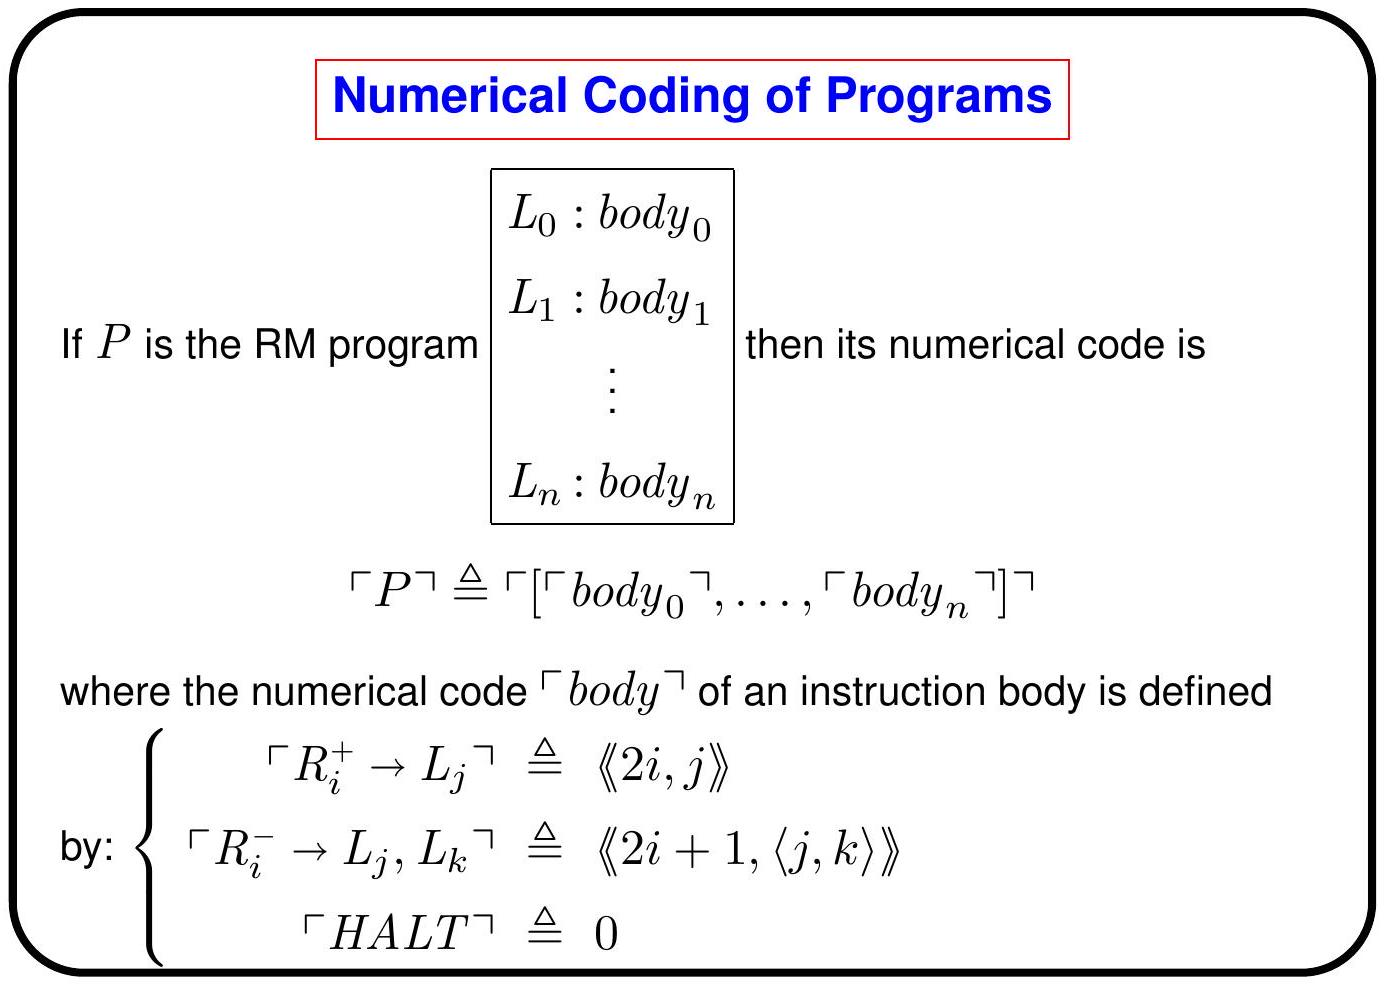
\includegraphics[max width=\textwidth, center]{2025_05_09_e840a83aab7eebacdc7fg-20}

Since $\langle-,-\rangle: \mathbb{N} \times \mathbb{N} \rightarrow \mathbb{N}^{+},\langle-,-\rangle: \mathbb{N} \times \mathbb{N} \rightarrow \mathbb{N}$ and $\ulcorner-\urcorner: \operatorname{List} \mathbb{N} \rightarrow \mathbb{N}$ are bijections, the functions $\ulcorner-\urcorner$ from bodies to natural numbers and $\ulcorner-\urcorner$ from RM programs to $\mathbb{N}$ are bijections.

Recall Addition $f(x, y) \triangleq x+y$ is Computable

Slide 27

\begin{center}
\begin{tabular}{|l|}
\hline
Registers \\
$R_{0} R_{1} R_{2}$ \\
Program \\
$L_{0}: R_{1}^{-} \rightarrow L_{1}, L_{2}$ \\
$L_{1}: R_{0}^{+} \rightarrow L_{0}$ \\
$L_{2}: R_{2}^{-} \rightarrow L_{3}, L_{4}$ \\
$L_{3}: R_{0}^{+} \rightarrow L_{2}$ \\
$L_{4}: H A L T$ \\
\hline
\end{tabular}
\end{center}

\begin{center}
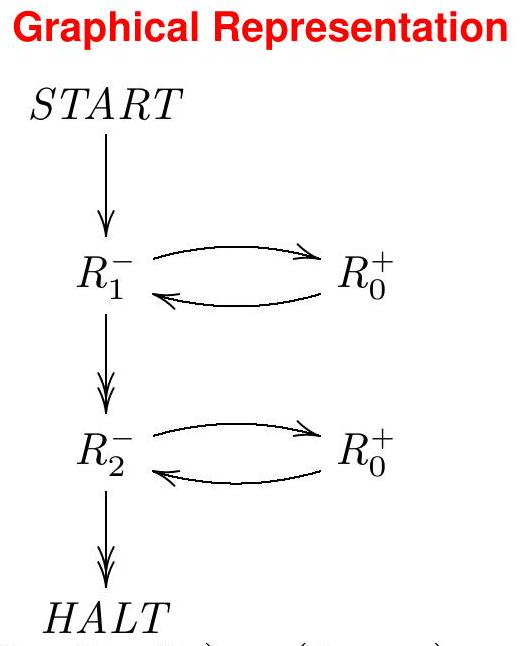
\includegraphics[max width=\textwidth]{2025_05_09_e840a83aab7eebacdc7fg-21}
\end{center}

If the machine starts with registers $\left(R_{0}, R_{1}, R_{2}\right)=(0, x, y)$, it halts with registers $\left(R_{0}, R_{1}, R_{2}\right)=(x+y, 0,0)$.

Slide 28

\section*{Coding of the RM for Addition}
$\ulcorner P\urcorner \triangleq\left\ulcorner\left[\left\ulcorner B_{0}\right\urcorner, \ldots,\left\ulcorner B_{4}\right\urcorner\right]\right\urcorner$ where

$$
\begin{aligned}
\left\ulcorner B_{0}\right\urcorner= & \left\ulcorner R_{1}^{-} \rightarrow L_{1}, L_{2}\right\urcorner=\langle(2 \times 1)+1,\langle 1,2\rangle\rangle \\
& =\langle\langle 3,9\rangle=8 \times(18+1)=152 \\
\left\ulcorner B_{1}\right\urcorner= & \left\ulcorner R_{0}^{+} \rightarrow L_{0}\right\urcorner=\langle 2 \times 0,0\rangle=1 \\
\left\ulcorner B_{2}\right\urcorner= & \left\ulcorner R_{2}^{-} \rightarrow L_{3}, L_{4}\right\urcorner=\langle\langle(2 \times 2)+1,\langle 3,4\rangle\rangle \\
= & \langle\langle 5,(8 \times 9)-1\rangle\rangle=\langle\langle 5,71\rangle \\
& =2^{5} \times((2 \times 71)+1)=32 \times 143=4576 \\
\left\ulcorner B_{3}\right\urcorner= & \left\ulcorner R_{0}^{+} \rightarrow L_{2}\right\urcorner=\langle 2 \times 0,2\rangle=5 \\
\left\ulcorner B_{4}\right\urcorner= & \ulcorner H A L T\urcorner=0
\end{aligned}
$$

In the next section, we will introduce the Universal Register Machine. The Universal Register Machine carries out the following computation: starting with $R_{0}=0, R_{1}=e$ (the code of the program), $R_{2}=a$ (code of the list of arguments), and all other registers zeroed:

\begin{itemize}
  \item decode $e$ as a RM program $P$
  \item decode $a$ as a list of register values $a_{1}, \ldots, a_{n}$
  \item carry out the computation of the RM program $P$ starting with $R_{0}=0, R_{1}=a_{1}, \ldots, R_{n}=a_{n}$ (and any other registers occurring in $P$ set to 0 ).\\
It is therefore important for you to understand what it means for a number $x \in \mathbb{N}$ to decode to a unique instruction $\operatorname{body}(x)$, and for a number $e \in \mathbb{N}$ to decode to a unique program $\operatorname{prog}(e)$.
\end{itemize}

\section*{Decoding Numbers as Bodies and Programs}
Any $x \in \mathbb{N}$ decodes to a unique instruction $\operatorname{bod} y(x)$ :\\
if $x=0$ then $\operatorname{bod} y(x)$ is HALT, else ( $x>0$ and) let $x=\langle\langle y, z\rangle$ in if $y=2 i$ is even, then $\operatorname{bod} y(x)$ is $R_{i}^{+} \rightarrow L_{z}$,\\
Slide 29 else $y=2 i+1$ is odd, let $z=\langle j, k\rangle$ in $\operatorname{body}(x)$ is $R_{i}^{-} \rightarrow L_{j}, L_{k}$\\
So any $e \in \mathbb{N}$ decodes to a unique program $\operatorname{prog}(e)$, called the register machine program with index $e$ :

$$
\left.\operatorname{prog}(e) \triangleq \left\lvert\, \begin{array}{c}
L_{0}: \operatorname{body}\left(x_{0}\right) \\
\vdots \\
L_{n}: \operatorname{body}\left(x_{n}\right)
\end{array}\right.\right] \text { where } e=\left\ulcorner\left[x_{0}, \ldots, x_{n}\right]\right\urcorner
$$

\section*{Example of $\operatorname{prog}(e)$}
\begin{itemize}
  \item $786432=2^{19}+2^{18}=0 \mathrm{~b} 11 \underbrace{0 \ldots 0}_{18{ }^{\prime \prime} 0^{0 " s}}=\ulcorner[18,0]\urcorner$
\end{itemize}

Slide 30

\begin{itemize}
  \item $18=0 \mathrm{~b} 10010=\langle 1,4\rangle=\left\langle\langle 1,\langle 0,2\rangle\rangle=\left\ulcorner R_{0}^{-} \rightarrow L_{0}, L_{2}\right\urcorner\right.$
  \item $0=\ulcorner H A L T\urcorner$
\end{itemize}

So $\operatorname{prog}(786432)=\begin{aligned} & L_{0}: R_{0}^{-} \rightarrow L_{0}, L_{2} \\ & L_{1}: H A L T\end{aligned}$

Notice that, when $e=0$, we have $0=\ulcorner[]\urcorner$ so $\operatorname{prog}(0)$ is the program with an empty list of instructions, which by convention we regard as a RM that does nothing (i.e. that halts immediately). Also, notice in slide 26 the jump to a label with no body (an erroneous halt). Again, choose some numbers and see what the register-machine programs they correspond to.


\end{document}